\documentclass[authoryear,preprint]{sigplanconf}

\usepackage{amsmath}
\usepackage{amsfonts}
\usepackage{amssymb}
\usepackage{amsthm}
\usepackage{algorithm2e}
\usepackage{listings}
\usepackage{xcolor}
\usepackage{tikz}
\usepackage{booktabs}
\usepackage{subfigure}
\usepackage[english]{babel}
\usepackage{blindtext}
\usetikzlibrary{shapes.geometric, arrows,chains}
\bibliographystyle{abbrvnat}
\usepackage{url}
\usepackage{hyperref}

\usepackage{color}

\definecolor{dkgreen}{rgb}{0,0.6,0}
\definecolor{gray}{rgb}{0.5,0.5,0.5}
\definecolor{mauve}{rgb}{0.58,0,0.82}
\usepackage{enumitem}
\newlist{steps}{enumerate}{1}
\setlist[steps, 1]{label = Step \arabic*:}

\lstset{frame=tb,
  language=Java,
  aboveskip=3mm,
  belowskip=3mm,
  showstringspaces=false,
  columns=flexible,
  basicstyle={\small\ttfamily},
  numbers=left,
  numberstyle=\tiny\color{gray},
  keywordstyle=\color{blue},
  commentstyle=\color{dkgreen},
  stringstyle=\color{mauve},
  breaklines=true,
  breakatwhitespace=true,
  tabsize=3
}

\begin{document}

\special{papersize=a4}
\setlength{\pdfpageheight}{\paperheight}
\setlength{\pdfpagewidth}{\paperwidth}


\title{Identifying Algorithmic Complexity Vulnerabilities Caused by
Input-Dependent Nested Loops}

\authorinfo{Mujahid Masood,Rafique Nazir}{mujahid.masood@stud.tu-darmstadt.de,rafique.nazir@stud.tu-darmstadt.de}{}
\maketitle

\section{Problem Statement}
\label{sec:problemstatement}

The single-threaded event model of JavaScript makes it vulnerable
to a specific class of denial of service attack called algorithmic
complexity attacks. These attacks consist of exploiting the worst
case performance of algorithms to trigger slow computations that
block the event loop for a large period of time. The focus of this
project is to identify function input-dependent nested loops by:
\begin{itemize}
\item Identifying the functions in code.
\item Identifying the input parameters of the functions.
\item Identifying the input-dependent nested loops inside the functions.
\item Analyzing the impact of function input-dependent loops in terms
of execution time as well as denial of service attack.
\end{itemize}


\section{Input dependent loops and execution time}
\label{sec:introduction}
Execution time of the functions is really important to write scalable applications. In normal application overall execution time of function depends upon the slowest function.

Consider the code in Listing \ref{l:iterate} in which we have an iterate function,with function input parameter max,which has a single loop,iterating up till max.

So caller of function can pass input of \begin{math} 10^{10} \end{math} and execution time of simple function with single loop will be around \textit{11s}.

\begin{lstlisting}[caption=iterate function with single loop,label=l:iterate,language=Java]

function iterate(max){

    var start = process.hrtime();
    var precision = 3;
    for(var i = 0; i< max; i++){
        var c = 10 + 5;
    }

    var elapsed = process.hrtime(start)[1] / 1000000;
    
	console.log(
		process.hrtime(start)[0] + " s, "+
		elapsed.toFixed(precision)+" ms - " 
	);
}

\end{lstlisting}

If other functions in application are taking less time, iterate
function is subject to performance bug and also security bug specially
in node modules.

This problems gets interesting if we introduce nested loops
i.e, 2 or 3 nested loops. Consider the code in Listing 2. Function
doubleLoop has input parameter max and two nested loops. Client
of doubleLoop can pass input max \begin{math} 10^{5} \end{math}
and can introduce a delay of around 6 seconds. Important thing to note is that function is
only doing simple sum of 10 and 5 but due to input dependent loop,
execution of the function takes longer time.

\begin{lstlisting}[caption=doubleLoop function with two nested loops,label=l:doubleLoop,language=Java]

function doubleLoop(max){

    var start = process.hrtime();
    var precision = 3;
    for(var i = 0; i< max; i++){
    	for(var j=0; j< i; j++){
			 var c = 10 + 5;
 		}
 	}

    var elapsed = process.hrtime(start)[1] / 1000000;
	console.log(
		process.hrtime(start)[0] + " s, "+
		elapsed.toFixed(precision)+" ms - " 
	);
}

doubleLoop(Math.pow(10,5));

\end{lstlisting}

As we increase the number of nested loops,to obtain longer execution time of function,we need to pass smaller function input parameter.For example a function with 3 nested loops and input parameter max
can have execution time of around 6 s with max = \begin{math} 10^{3.2} \end{math}
Consider the code in Listing \ref{l:tripleLoop}.

\begin{lstlisting}[caption=tripleLoop function with three nested loops,label=l:tripleLoop,language=Java]
function tripleLoop(max){
    var start = process.hrtime();
    var precision = 3;
    for(var i = 0; i< max; i++){
    	for(var j=0; j< i; j++){
    		for(var k=0; k< max; k++){
				 var c = 10 + 5;
 			}
 		}
 	}

    var elapsed = process.hrtime(start)[1] / 1000000;
	console.log(
		process.hrtime(start)[0] + " s, "+
		elapsed.toFixed(precision)+" ms - " 
	);
}

tripleLoop(Math.pow(10,3.2));

\end{lstlisting}


\section{Problems with using Function Input-Dependent Loops}
\label{sec:problems}
Code in Listing \ref{l:doubleLoop} and Listing \ref{l:tripleLoop} are not only subject to performance issues but also to denial of service (DoS) attacks. Attacker can control the input parameter and can introduce delay of 10-15 seconds in the execution time of function. Node.js security experts consider any slowdown larger than one second as security relevant.

\section{Avoiding the problem}
\label{sec:avoiding}

Following are some approaches which can be used to avoid the problem with input dependent nested loops.

\subsection{Approach 1 : Introduce Upper bound on input parameters}
One simple way to avoid such problem is introducing upper bound on input parameter.
Consider the code in Listing \ref{l:avoidProblem} which exits from the function if input exceeds the given bound which is \begin{math} 10^{2} \end{math}.

\begin{lstlisting}[caption=avoidProblem function with 3 nested loops and upper bound on input parameter,label=l:avoidProblem,language=Java]

function avoidProblem(max){
	if(max > Math.pow(10,2)) {
		return;	
	}
    for(var i = 0; i< max; i++){
    	for(var j=0; j< i; j++){
    		for(var k=0; k< max; k++){
				 var c = 10 + 5;
 			}
 		}
 	}
}

avoidProblem(Math.pow(10,3.2));

\end{lstlisting}

\subsubsection{Problems with Approach 1}

Introducing such input bound checks as in Listing \ref{l:avoidProblem} requires full understanding of the code and also the usage of function.

\subsection{Approach 2 : Changing the logic} 
Other way can be changing the logic from nested loops to maybe introducing new functions, which means one needs to find places in the code where input-dependent nested loops are used, for example not using nested loops.
\subsubsection{Problems with Approach 2}
\begin{itemize}
\item Code is already deployed in production environment.
\item JavaScript uses minified versions of files therefore it is difficult to find code usage.
\item JavaScript file can have 10000s lines of code,finding such occurrences in code can be difficult.
\item Different variations of functions:
		\begin{itemize}
			\item JavaScript can use assignment of function to other variable 
				e.g, var a = function() {}
			\item Using anonymous functions
				e.g, (function())
			\item JavaScript also uses nested functions
				e.g, (function(a, function(){}))
		\end{itemize}
\item Different variations of Loops
	 e.g  For, While, For In, forEach etc.
\item Assignment of function input parameter to other variables and using that in loop.
\item Using input parameter in function call which in turn is used in loops.
			
\end{itemize}

\section{Our Approach}
\subsection{High Level Steps}
\begin{itemize}
	\item Statically analyse JavaScript code.
	\item Find out if code uses function.
	\item Find out if function uses input parameters.
	\item Find out if function uses loops.
	\item Find out if loops use function input parameters directly or indirectly.
	\item Write vulnerable output.
	\item Validate the results.
			\begin{itemize}
				\item Manually trigger the identified function.
				\item Calculate the execution time of function on different inputs
			\end{itemize}
\end{itemize}

\subsection{Implementation Technologies}
\begin{itemize}
	\item Static Analyser : Google Closure Compiler for static analysis.
	\item Programming Language : Java 8
	\item Build tool : Maven
	\item Bash Script (Utility)
			\begin{itemize}
				\item clone.sh : cloning git code to specified directory
				\item search.sh: Bash script to search JavaScript Projects on Github, opens the browser session for displaying results.\end{itemize}
\end{itemize}


\subsection{Implementation: Detailed Steps}

Figure \ref{f:workflow} shows the implementation details.
\begin{figure}[ht]
\centering
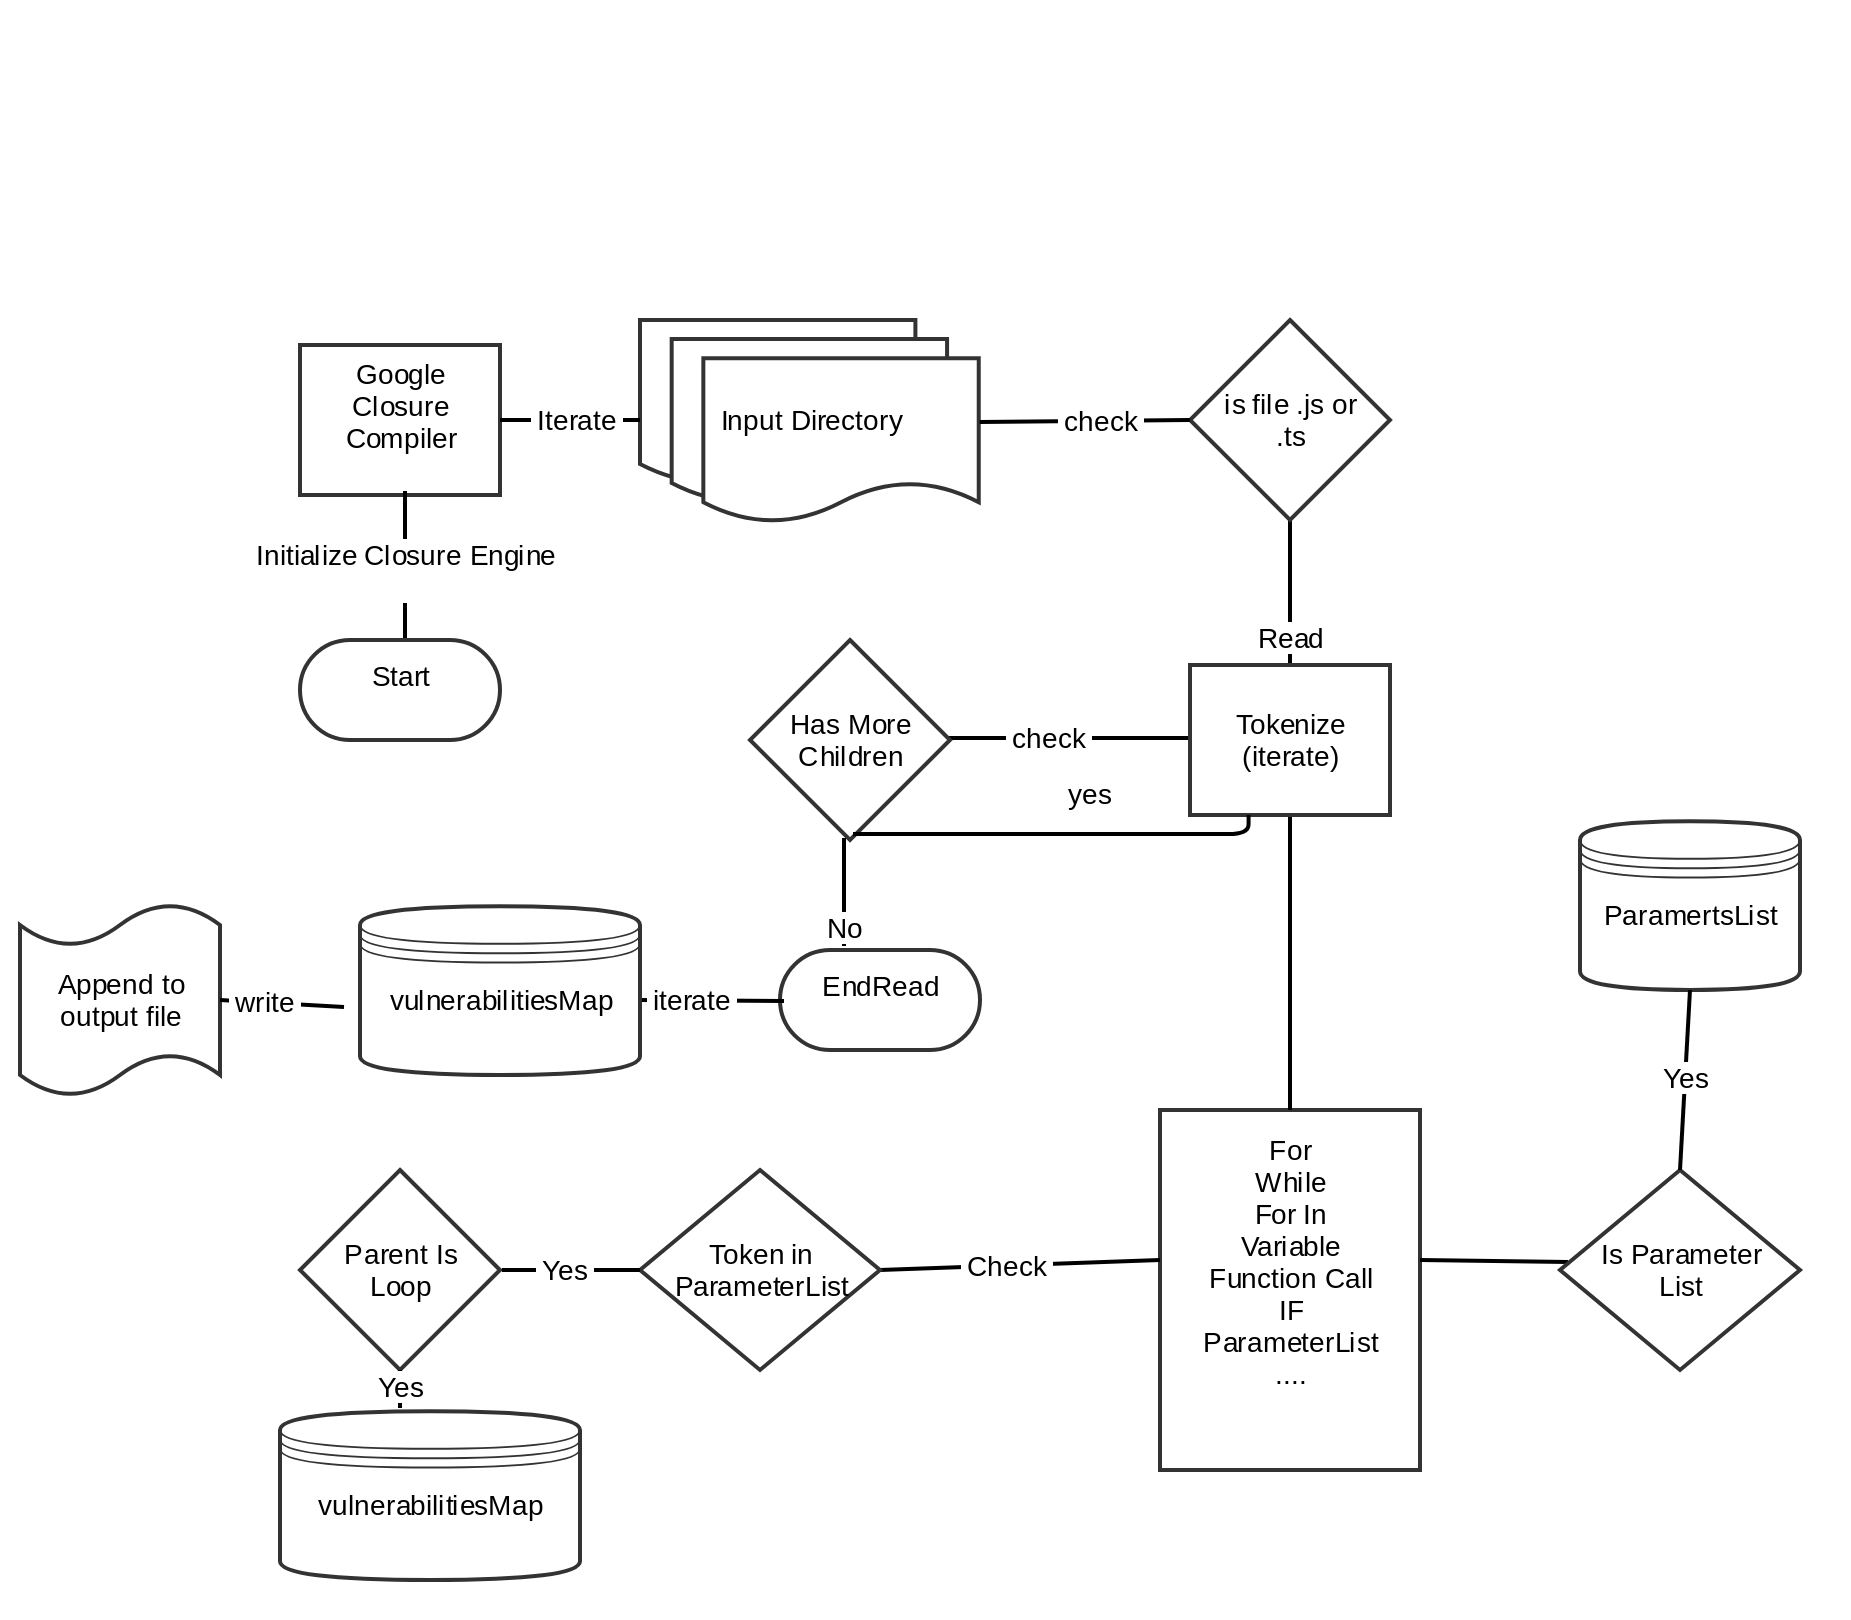
\includegraphics[height=8cm]{figures/workflow}
\caption[Implementation Detail]{\label{f:workflow}Implementation Detail.}
\end{figure}

\begin{itemize}
\item Iterate through the directory.
\item Check for any .js or .ts file.
\item Initialize Google Closure Engine.
\item Read the JavaScript File.
\item Tokenize the JavaScript code.
\item Iterate through the tokens.
\item Check if the token is function, save the reference for future use.
\item Check if token is the parameterList, add it in parameter list.
\item Check if the variable is present in parameter list.
\item Check if the parent of variable is loop (while, for, forEach, for in).
\item If parent of variable is loop and present in parameters, add it into vulnerabilitiesMap.
\item After traversing all tokens in file, print the output in text file.
\end{itemize}

\subsection{Project Structure}

\begin{figure}[ht]
\centering
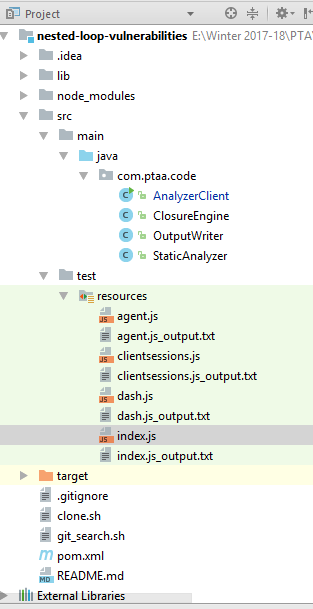
\includegraphics[width=1\linewidth]{figures/project-structure}
\caption[Project Structure]{\label{f:structure}Project Structure.}
\end{figure}

\begin{itemize}
\item lib : This folder contains jar files.
\item node modules : This folder contains the npm modules on which we have performed the analysis.
\item src : Contains the source code (Java Classes), actual code with implemented logic.
	\begin{itemize}
		\item main
			\begin{itemize}
		\item AnalyzerClient : Main class to invoke the StaticAnalyser.
		\item ClosureEngine : Class for Google closure related settings, mainly initializes the Google Closure Compiler.
		\item OutputWriter : Class to write the output vulnerabilities in text file.
		\item StaticAnalyzer : Class has main logic, iterates the JavaScript code, checks for functions, loops and decides vulnerabilities.\end{itemize}
		
		\item test
			\begin{itemize}
				\item resources : Contains our test cases and output files.
			\end{itemize}
		
	\end{itemize}

\item .gitignore : Contains git ignored files.
\item clone.sh : Bash script to clone the git repository to specified location.
	\begin{itemize}
		\item It takes two input parameters 1. repository and 2. location where to clone the project
		\\
		clone.sh can be run as shown below\\
		
		sh clone.sh https://github.com/project.git /node modules \\
		
		It will create new folder named project.git under node modules directory and clone the project from given online location.
		
	\end{itemize}

\item search.sh : Searches the JavaScript projects on github, to display the results it opens google chrome browser.

\item pom.xml : It contains maven related configurations.
\item README.md : Contains the instructions on how to use project.
		
\end{itemize}

\section{Results}
Following section discusses the results on our own test cases and also on node modules.
In Project code index.js under resources folder contains our test cases, we will demonstrate a few from index.js file.

\begin{figure}[ht]
\centering
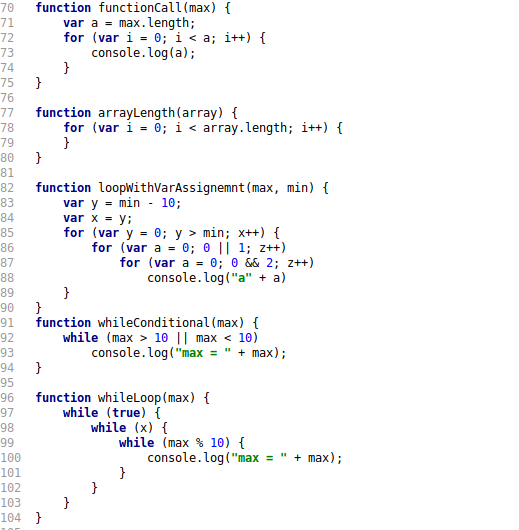
\includegraphics[width=1\linewidth]{figures/testcases}
\caption[Manual Tests]{\label{f:testcases}Manual Tests.}
\end{figure}

From the figure 3. we expect to find vulnerabilities on lines 72,78, 85, 92 and 99 because the functions use input dependent loops.
We ran the tests using our code and output is as shown in figure 4.
\subsection{Manual Tests}

\begin{figure}[ht]
\centering
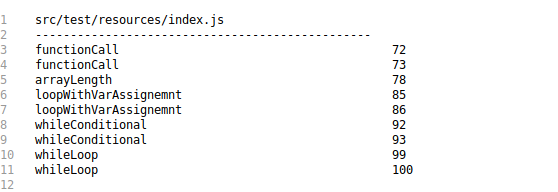
\includegraphics[width=1\linewidth]{figures/output}
\caption[Output of Manual Tests]{\label{f:testcases}Output of Manual Tests.}
\end{figure}

As we can see our code correctly identifies the specified lines where possible vulnerabilities can occur along with some false positives.
Output format is
\begin{itemize}
\item First line is file name for which analysis is done.
\item Multiple dashes for separation.
\item Subsequent lines shows function name in left column and line number in right column. In case of anonymous function output function on left is null.

\end{itemize}

\subsubsection{Validation}
With above functions validation is easy, we added execution time to validate our claim as shown in Listing \ref{l:doubleLoop}, \ref{l:tripleLoop}

\section{Analysing Node modules}
In order to identify nested loops we mainly focused on video streaming,audio streaming, matrix and data structure libraries to find the code using input dependent nested loops.
We found nested loops inside.
All these libraries and simulations are inside node modules folder.
\begin{itemize}
\item tough-cookie
\item dashjs
\item loaddash
\end{itemize}

We identified vulnerabilities in other npm modules with single loop.
All these simulations are inside resources folder of project.
\begin{itemize}
\item useragent
\item clientsession
\item glmatrix
\end{itemize}


We performed our analysis on following node modules.

Table~\ref{t:Comparison} shows how a table looks like.

\begin{table}[h]
\small
\begin{tabular}{ |p{1.9cm}||p{1.9cm}|p{1.9cm}|p{1.9cm}|  }
 \hline
 \textbf{Node Module}&\textbf{Has Nested Loops}&\textbf{Found Vulnerabilities} &\textbf{False Positives}\\
 \hline
loaddash&yes&yes &yes  \\
\hline 
dashjs&yes&yes&yes  \\
\hline 
useragent &no&yes &yes  \\
\hline 
 tough-cookie & yes&yes &yes \\
\hline 

\end{tabular}

\caption[Comparison]{\label{t:Comparison} Result of analyzing node modules.}
\end{table}
\subsection{UserAgent Results}
\begin{figure}[ht]
\centering
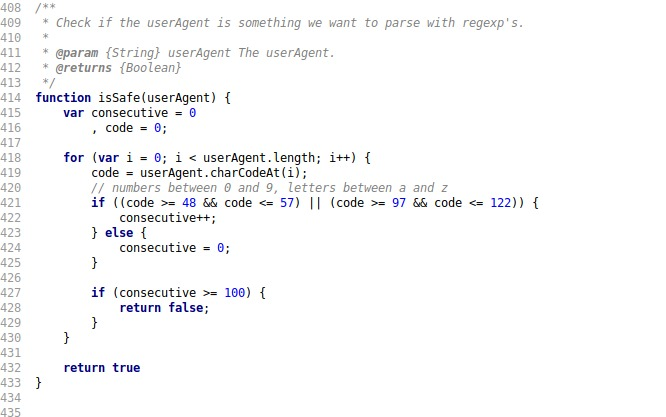
\includegraphics[height=5cm]{figures/useragent-isSafe}
\caption[Code analysis performed on node module useragent isSafe function]{\label{f:isSafe}Node module useragent isSafe function}
\end{figure}

In above figure \ref{f:isSafe} code on line numbers 418 and 419 is vulnerable.After running our code we identified our code on node module user agent we identified  the results as shown in the figure \ref{f:isSafe}

\subsection{Validating UserAgent Results}
We added the code to calculate execution time of function in the start and end of parse function as shown in Listing \ref{l:parse}
 
\begin{lstlisting}[caption=Code Instrumentation,label=l:parse,language=Java]

/**
 * Parses the user agent string with the generated parsers from the
 * ua-parser project on google code.
 *
 * @param {String} userAgent The user agent string
 * @param {String} [jsAgent] Optional UA from js to detect chrome frame
 * @returns {Agent}
 * @api public
 */
var process = require('process');
var precision = 3;
exports.parse = function parse(userAgent, jsAgent) {
    var start = process.hrtime();
  if (!userAgent || !isSafe(userAgent)) return new Agent();

  var length = agentparserslength
    , parsers = agentparsers
    , i = 0
    , parser
    , res;

  for (; i < length; i++) {
    if (res = parsers[i][0].exec(userAgent)) {
      parser = parsers[i];

      if (parser[1]) res[1] = parser[1].replace('$1', res[1]);
      if (!jsAgent) return new Agent(
          res[1]
        , parser[2] || res[2]
        , parser[3] || res[3]
        , parser[4] || res[4]
        , userAgent
      );

      break;
    }

      var elapsed = process.hrtime(start)[1] / 1000000;
      console.log(process.hrtime(start)[0] + " s, " + elapsed.toFixed(precision) + " ms - " );
  }

\end{lstlisting}



\subsection{Manually Triggering Identified Vulnerable Function}

A random test script of length  \begin{math}10^{4} \end{math} was provided as an input to a parse function and it took approximately 7 seconds to execute the method as shown in listing \ref{l:test} below:

\begin{lstlisting}[caption=Manual Triggering of vulnerable function in npm module useragent,label=l:test,language=Java]

var useragent = require('useragent');
useragent(true);
var req = {}
var string = ''
for(var i=0; i< Math.pow(10,4); i++){
    string += i + " ";
}

req.headers = {'user-agent': string}
req.query = {'jsuseragent':'ok'}
var agent2 = useragent.parse(req.headers['user-agent'], req.query.jsuseragent);

\end{lstlisting}

\subsection{tough-cookie Results}

\begin{figure}[ht]
\centering{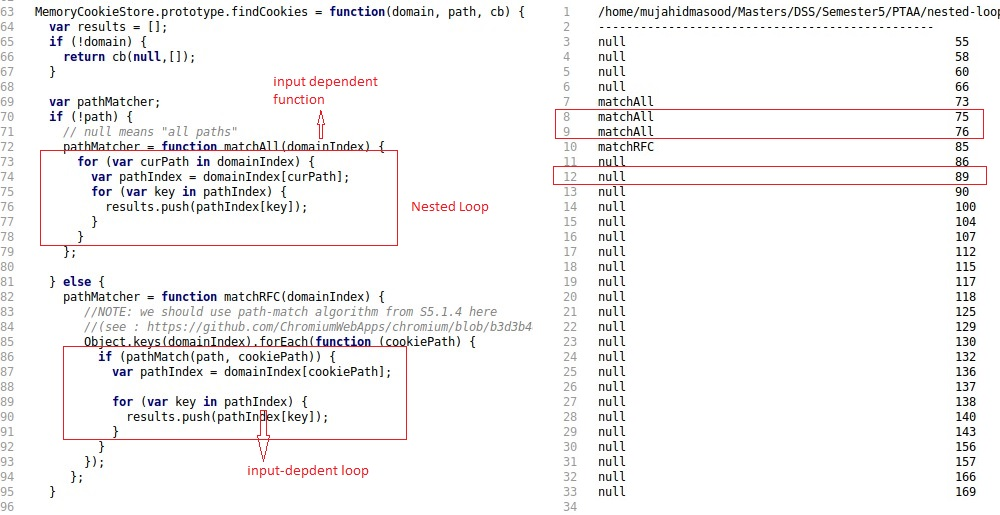
\includegraphics[height=5cm]{figures/tough-cookie}}
\caption[vulnerablilities in npm module tough-cookie in file lib/memstore.js]{\label{f:cookie}vulnerabilities in npm module tough-cookie in file lib/memstore.js}
\end{figure}

We found nested loops in tough-cookie as shown in figure \ref{f:cookie}.

\section{Conclusion}

This project correctly analyses the vulnerabilities along with 80 percentage of false positives. 

\subsection{Reason for false positives}
Our implementation checks if the input parameter is used, if it is used at any instance of variable, function call or assignment, we output it as vulnerable. This is not the scope of project but technically some function call can make take much longer time for execution because of used parameter.

\section{Future Work}
\begin{itemize}
\item Reducing the number of false positives in the code this can be done by properly defining and documenting vulnerabilities. For example if we have 3 nested functions and all have parameters but inner function as loop which uses parameters, should this be considered vulnerable or not.
\item Writing the bash or python script to make the search code with nested loop instances easy to find on github or other code repositories.
for example \\
 \textit{git grep -l --all-match -e "for" --or -e "while"} \\
this command find for or while loop instance in code.
\item Validating the code is bit challenging because vulnerable function can be dependent on many other calling functions and to really see it in practice one needs to fulfil all dependencies.


\end{itemize}

\section{Difficulties and Challenges}

Following are some places we found it difficult
\begin{itemize}
\item The code instances which use nested loops.
\item Triggering the identified code because functions identified had many dependencies.
\item Coming up with input parameter, we solved this by creating random input in case of useragent.
\end{itemize}

\end{document}